{\bf Introduction}

This homework is a series of multiple choice questions focusing on Machine
Learning theory.  It includes a short, fictitious case study, some statistical
theory revolving around the bias-variance tradeoff, and even a look into
interesting new Machine Learning research!

{\bf How to submit:}  This assignment includes only multiple choice questions.
Even though these are not coding questions, you will submit your response to
each question in the |submission.py| file.  The response to the first question
looks like this:

\begin{center}
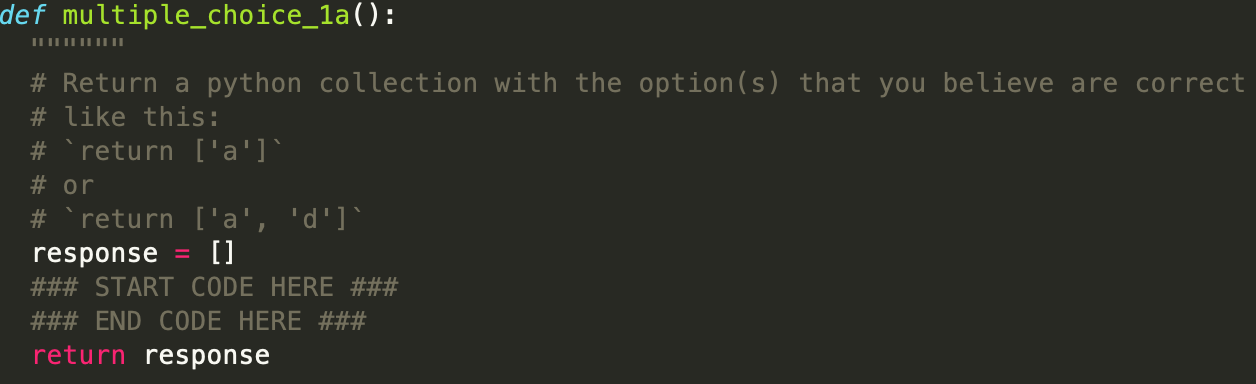
\includegraphics[width=1\textwidth]{sample_question_empty.png}
\end{center}

If you believe that |a| and |b| are the correct responses to this question, you
will type |response = [`a', `b']| between the indicated lines like this:

\begin{center}
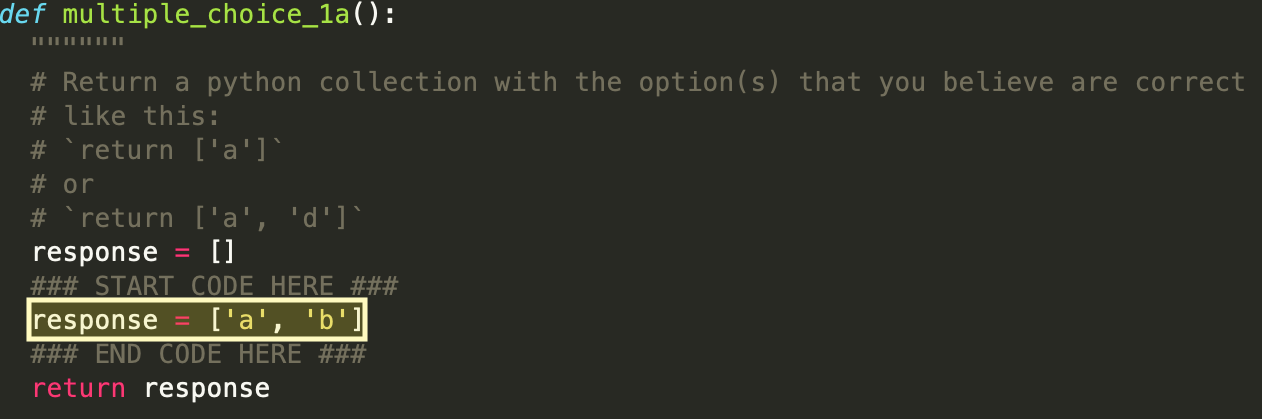
\includegraphics[width=1\textwidth]{sample_question_complete.png}
\end{center}

{\bf How to verify your submission:}
You can run the student version of the autograder locally like all coding
problem sets.  In the case of this problem set, the helper tests will verify
that your responses are within the set of possible choices for each question
(e.g. the helper functions will flag if you forget to answer a question of if
you respond with |[`a', `d']| when the choices are |[`a', `b', `c']|.)  See the
previous page for instructions to run the autograder.
